\documentclass[border=0.2cm]{standalone}
%
% AUTHOR: Nicolás Otero Martínez - nom05 (at) uvigo.es.
% COLLABORATORS: -
% MIT License in the corresponding file.
% This LaTeX code employs `memoir' class.
% Used as reference: https://latexdraw.com/draw-flowcharts-latex-tutorial/
%
\usepackage{tikz}
\usetikzlibrary{shapes,positioning}

\begin{document}
	
	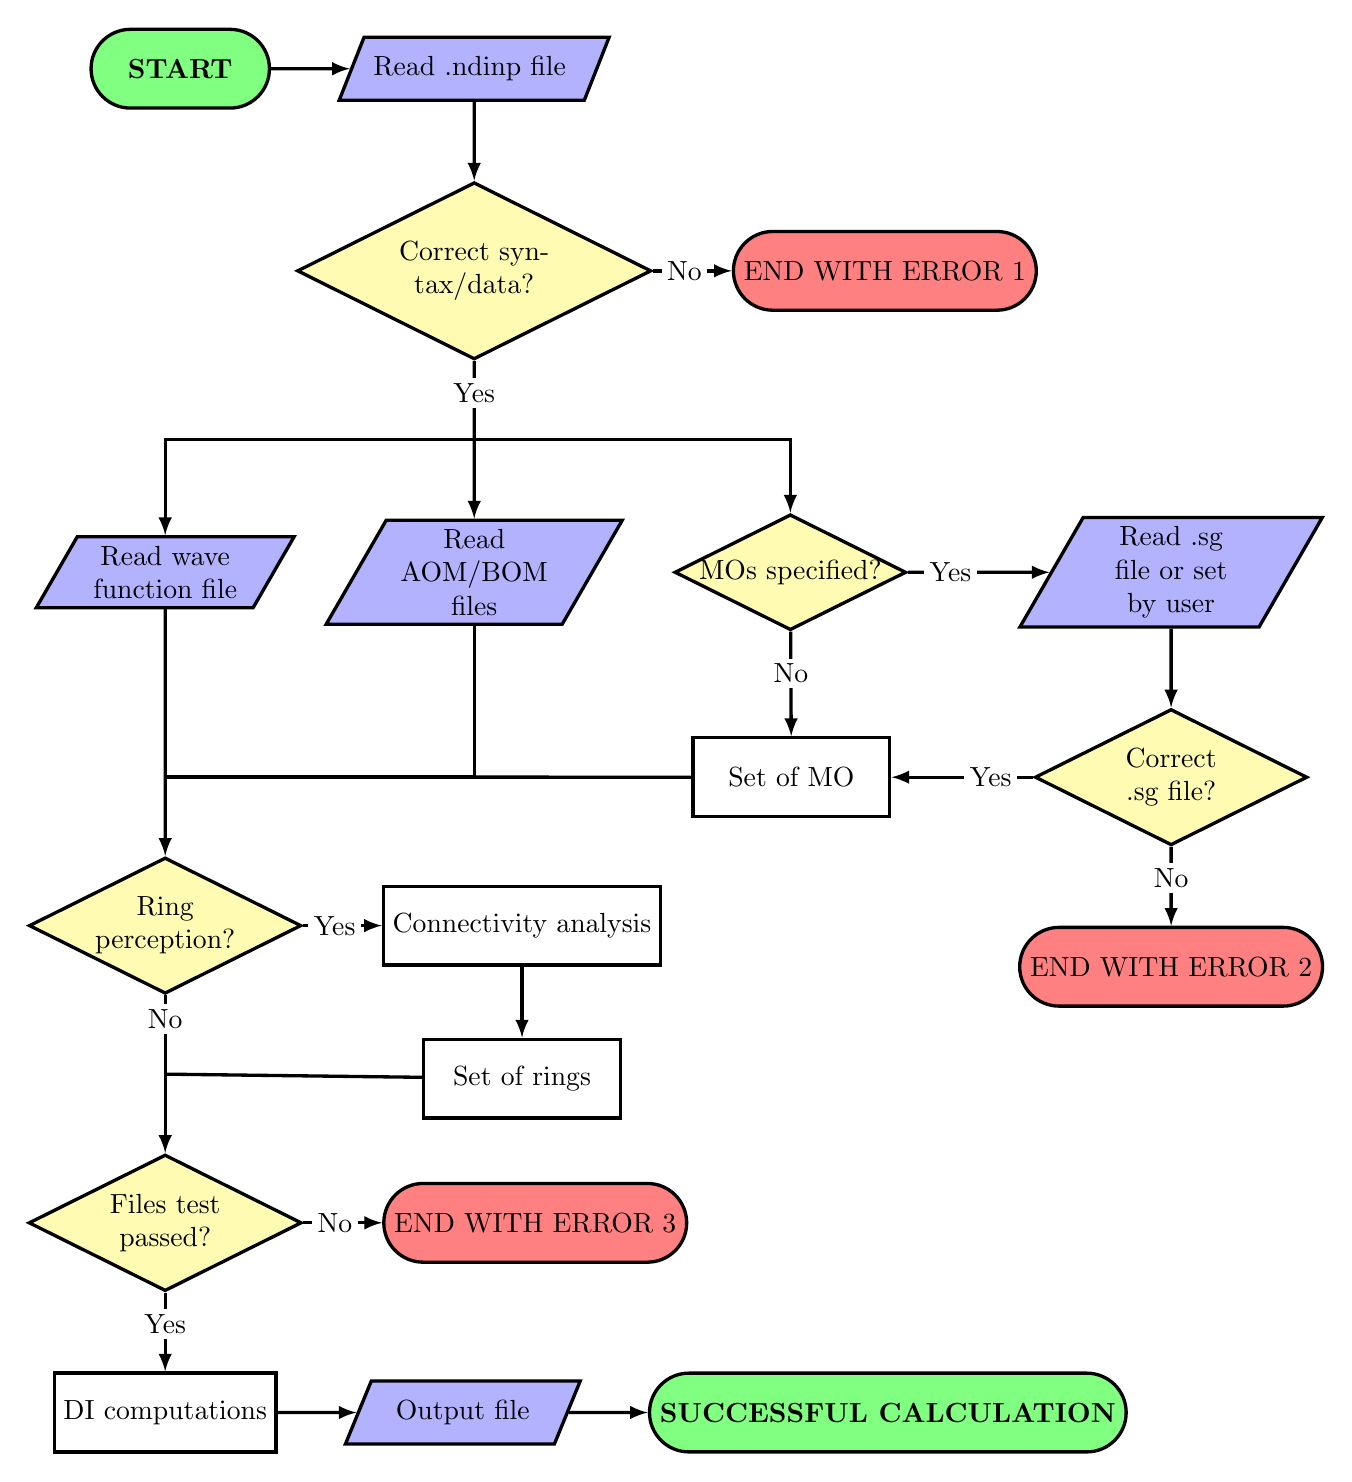
\begin{tikzpicture}[font=\normalsize,very thick,align=center]
		
		% Start block
		\node[
			draw,
			fill=green!50,
			rounded rectangle,
			minimum width=2.5cm,
			minimum height=1cm
		] (start) {\textbf{START}};
		
		% Read input file
		\node[
			draw,
			trapezium, 
			trapezium left angle = 60,
			trapezium right angle = 120,
			trapezium stretches,
			minimum width=3.cm,
			minimum height=.8cm,
			fill=blue!30,
			right=of start
		] (inputfile) { Read .ndinp file };
		
  		% Verifying input syntax
		\node[
			draw,
			diamond,
			aspect=2,
			minimum width=2.cm,
			text width=3cm,
			text centered,
			inner sep=0,
			fill=yellow!30,
			below=of inputfile
		] (syntaxinput) {Correct syntax/data?};
		
		\node[coordinate,below=of syntaxinput] (ghostsyntax) {};

		% Syntax Error 
		\node[
			draw,
			rounded rectangle,
			fill=red!50,
			minimum width=2.5cm,
			minimum height=1cm,
			right=of syntaxinput
		] (syntaxerror) {END WITH ERROR 1};
		
		% Read AOM/BOM files
		\node[
			draw,
			trapezium, 
			trapezium left angle = 60,
			trapezium right angle = 120,
			trapezium stretches,
			minimum width=3.cm,
			minimum height=.8cm,
			text width=2cm,
			fill=blue!30,
			below=of ghostsyntax
		] (aomfiles) {Read AOM/BOM files};
		
		% Read wave function
		\node[
			draw,
			trapezium, 
			trapezium left angle = 60,
			trapezium right angle = 120,
			trapezium stretches,
			minimum width=3.cm,
			minimum height=.8cm,
			text width=2cm,
			fill=blue!30,
			left=of aomfiles
		] (wffile) {Read wave function file};
		
		\node[coordinate,above=.1cm of wffile] (fixwffile) {};
		
		% Sigma/pi separation request
		\node[
			draw,
			diamond,
			aspect=2,
			fill=yellow!30,
			minimum width=2.5cm,
			inner sep=0,
			right=of aomfiles
		] (sigmapi) {MOs specified?};
		
		% Read .sg file
		\node[
			draw,
			trapezium, 
			trapezium left angle = 60,
			trapezium right angle = 120,
			trapezium stretches,
			minimum width=3.cm,
			minimum height=.8cm,
			fill=blue!30,
			text width=2cm,
			right=1.8cm of sigmapi
		] (readsg) {Read .sg file or set by user};
		
		% Correct .sg file?
		\node[
			draw,
			diamond,
			minimum width=2.5cm,
			inner sep=0,
			text width=2cm,
			aspect=2,
			fill=yellow!30,
			below=of readsg
		] (checksg) {Correct .sg file?};
		
		% Error: .sg file
		\node[
			draw,
			rounded rectangle,
			fill=red!50,
			minimum width=2.5cm,
			minimum height=1cm,
			below=of checksg
		] (sgerror) {END WITH ERROR 2};
		
		% Set of MOs defined
		\node[
			draw,
			minimum width=2.5cm,
			minimum height=1cm,
			left=1.8cm of checksg
		] (MOset) {Set of MO};

		% Ghost point
		\node[coordinate,below=2.13cm of wffile] (ghostwf) {};

		% Ring perception?
		\node[
			draw,
			diamond,
			minimum width=2.5cm,
			inner sep=0,
			text width=2cm,
			aspect=2,
			fill=yellow!30,
			below=of ghostwf
		] (ringperception) {Ring perception?};

		% Ghost point
		\node[coordinate,below=of ringperception] (ghostring) {};
		
		% Connectivity analysis
		\node[
			draw,
			minimum width=2.5cm,
			minimum height=1cm,
			right=of ringperception,
		] (connect) {Connectivity analysis};
		
		% All files exist and correct?
		\node[
			draw,
			diamond,
			minimum width=2.5cm,
			text width=2cm,
			aspect=2,
			fill=yellow!30,
			inner sep=0,
			below=of ghostring,
		] (goodfiles) {Files test passed?};
		
		% Files Error 
		\node[
			draw,
			rounded rectangle,
			fill=red!50,
			minimum width=2.5cm,
			minimum height=1cm,
			right=of goodfiles
		] (fileserror) {END WITH ERROR 3};
		
		% Set of rings
		\node[
			draw,
			minimum width=2.5cm,
			minimum height=1cm,
			below=.9cm of connect
		] (rings) {Set of rings};
		
		% Computation of N-delocalization indices
		\node[
			draw,
			minimum width=2.5cm,
			minimum height=1cm,
			below=of goodfiles
		] (DI) {DI computations};
		
		% Computation of N-delocalization indices
		\node[
			draw,
			trapezium,
			trapezium left angle = 60,
			trapezium right angle = 120,
			trapezium stretches,
			minimum width=3.cm,
			minimum height=.8cm,
			text width=2cm,
			fill=blue!30,
			right=of DI
		] (output) {Output file};
		
		% Start block
		\node[
			draw,
			rounded rectangle,
			very thick,
			fill=green!50,
			minimum width=2.5cm,
			minimum height=1cm,
			right=of output
		] (success) {\textbf{SUCCESSFUL CALCULATION}};
		
		% Arrows
		\draw[-latex] 
				(start)				edge 												(inputfile)
				(inputfile) 		edge 												(syntaxinput)
				(syntaxinput) 		edge 												(aomfiles)
				(readsg) 			edge 												(checksg)
				(connect) 			edge 												(rings)
				(DI) 				edge 												(output)
				(output) 			edge 												(success)
				(aomfiles) 			|- 	 												(ghostwf)
				(wffile) 			edge 												(ringperception)
				(ghostsyntax) 		-|	 												(sigmapi);
		\draw[-latex]
				(ghostsyntax) 		-|	 												(wffile);
		\draw[-latex]
				(syntaxinput) 		edge node[pos=0.4 ,fill=white,inner sep=2pt]{No}	(syntaxerror)
				(checksg) 			edge node[pos=0.4 ,fill=white,inner sep=2pt]{No}	(sgerror)
				(sigmapi) 			edge node[pos=0.4 ,fill=white,inner sep=2pt]{No}	(MOset)
				(ringperception) 	edge node[pos=0.15,fill=white,inner sep=2pt]{No}	(goodfiles)
				(goodfiles) 		edge node[pos=0.4 ,fill=white,inner sep=2pt]{No}	(fileserror);
		\draw[-latex] 
				(sigmapi)			edge node[pos=0.3 ,fill=white,inner sep=2pt]{Yes}	(readsg)
				(checksg) 			edge node[pos=0.3 ,fill=white,inner sep=2pt]{Yes}	(MOset)
				(ringperception)	edge node[pos=0.4 ,fill=white,inner sep=2pt]{Yes}	(connect)
				(goodfiles)			edge node[pos=0.4 ,fill=white,inner sep=2pt]{Yes}	(DI);
		\draw 	(syntaxinput) 		edge node[pos=0.4 ,fill=white,inner sep=2pt]{Yes}	(ghostsyntax);
		\draw 	(rings) 			edge 												(ghostring)
				(wffile)			edge												(ghostwf)
				(MOset)				edge												(ghostwf);

		% Text and nodes:
		% * (start) {START};
		% * (inputfile) { Read .ndinp file };
		% * (syntaxinput) {Correct syntax/data?};
		% * (ghostsyntax) {};
		% * (syntaxerror) {END WITH ERROR 1};
		% * (aomfiles) {Read AOM/BOM files};
		% * (wffile) {Read wave function file};
		% * (fixwffile) {};
		% * (sigmapi) {$\sigma$/$\pi$ MOs?};
		% * (readsg) {Read .sg file};
		% * (checksg) {Correct .sg file?};
		% * (sgerror) {END WITH ERROR 2};
		% * (MOset) {Set of MO};
		% * (ghostwf) {};
		% * (ringperception) {Ring perception?};
		% * (ghostring) {}
		% * (connect) {Connectivity analysis};
		% * (goodfiles) {Files test passed?};
		% * (fileserror) {END WITH ERROR 3};
		% * (rings) {Set of rings};
		% * (DI) {DI computation};
		% * (output) {Output file};
		% * (success) {SUCCESSFUL CALCULATION};
		
	\end{tikzpicture}
	
\end{document}